%----------------------------------------------------------------------------------------
%	PACKAGES AND OTHER DOCUMENT CONFIGURATIONS
%----------------------------------------------------------------------------------------

\documentclass[paper=a4, fontsize=11pt]{scrartcl} % A4 paper and 11pt font size

% ---- Entrada y salida de texto -----

\usepackage[T1]{fontenc} % Use 8-bit encoding that has 256 glyphs
\usepackage[utf8]{inputenc}
%\usepackage{fourier} % Use the Adobe Utopia font for the document - comment this line to return to the LaTeX default

% ---- Idioma --------

\usepackage[spanish, es-tabla]{babel} % Selecciona el español para palabras introducidas automáticamente, p.ej. "septiembre" en la fecha y especifica que se use la palabra Tabla en vez de Cuadro

% ---- Otros paquetes ----
\usepackage{csquotes} %Para permitir el uso de comillas Quotes https://tex.stackexchange.com/questions/36812/isnt-there-any-other-way-of-doing-double-quotes-in-latex-besides
\usepackage[hyphens]{url} % ,href} %para incluir URLs e hipervínculos dentro del texto (aunque hay que instalar href)
\usepackage{hyperref}
\usepackage{color}
\usepackage{graphics,graphicx, floatrow} %para incluir imágenes y notas en las imágenes
\usepackage{graphics,graphicx, float} %para incluir imágenes y colocarlas

\graphicspath {{./img/}}

\usepackage{listings}  %para introducir comandos

\lstdefinestyle{mybash}
{basicstyle=\ttfamily,
  showstringspaces=false,
  commentstyle=\color{red},
  keywordstyle=\color{blue},
  language=bash,
  alsoletter=/,
  basicstyle=\footnotesize,
  numbers=left,
  stepnumber=1,
  showstringspaces=false,
  tabsize=1,
  breaklines=true,
  breakatwhitespace=false,
}
\lstdefinestyle{mysql}
{basicstyle=\ttfamily,
  showstringspaces=false,
  commentstyle=\color{red},
  keywordstyle=\color{blue},
  language=sql,
  basicstyle=\footnotesize,
  numbers=left,
  stepnumber=1,
  showstringspaces=false,
  tabsize=1,
  breaklines=true,
  breakatwhitespace=false,
}


% Para hacer tablas comlejas
%\usepackage{multirow}
%\usepackage{threeparttable}

%\usepackage{sectsty} % Allows customizing section commands
%\allsectionsfont{\centering \normalfont\scshape} % Make all sections centered, the default font and small caps

\usepackage{fancyhdr} % Custom headers and footers
\pagestyle{fancyplain} % Makes all pages in the document conform to the custom headers and footers
\fancyhead{} % No page header - if you want one, create it in the same way as the footers below
\fancyfoot[L]{} % Empty left footer
\fancyfoot[C]{} % Empty center footer
\fancyfoot[R]{\thepage} % Page numbering for right footer
\renewcommand{\headrulewidth}{0pt} % Remove header underlines
\renewcommand{\footrulewidth}{0pt} % Remove footer underlines
\setlength{\headheight}{13.6pt} % Customize the height of the header

\setlength\parindent{0pt} % Removes all indentation from paragraphs - comment this line for an assignment with lots of text

\newcommand{\horrule}[1]{\rule{\linewidth}{#1}} % Create horizontal rule command with 1 argument of height


%----------------------------------------------------------------------------------------
%	TÍTULO Y DATOS DEL ALUMNO
%----------------------------------------------------------------------------------------
\graphicspath{ {img/} }

\title{
\normalfont \normalsize

\includegraphics[width=6cm,height=6cm]{logo}\\
\textsc{\textbf{Bootcamp Especialidad GNU/Linux (2023)}} \\ [25pt] % Your university, school and/or department name(s)
\horrule{0.5pt} \\[0.4cm] % Thin top horizontal rule
\huge Lab 11 - Creación de túneles PPTP con Wireguard \\ % The assignment title
\horrule{2pt} \\[0.5cm] % Thick bottom horizontal rule
}


%https://es.overleaf.com/learn/latex/Inserting_Images
%Ruta relativa de   imagenes

\author{Pedro Antonio Mayorgas Parejo} % Nombre y apellidos

\date{\normalsize\today} % Incluye la fecha actual

%----------------------------------------------------------------------------------------
% DOCUMENTO
%----------------------------------------------------------------------------------------

\begin{document}

\maketitle % Muestra el Título

\newpage %inserta un salto de página

\tableofcontents % para generar el índice de contenidos

\newpage

%----------------------------------------------------------------------------------------
%	Cuestión 1
%----------------------------------------------------------------------------------------

\section{Topología}

Tenemos la siguiente topología, donde tenemos conectados a través de un switch de L2, dos pfsense que hacen de doble funcionalidad, de router y de firewall. Así como a los host finales que consisten en un

\begin{figure}[H]
	\centering
	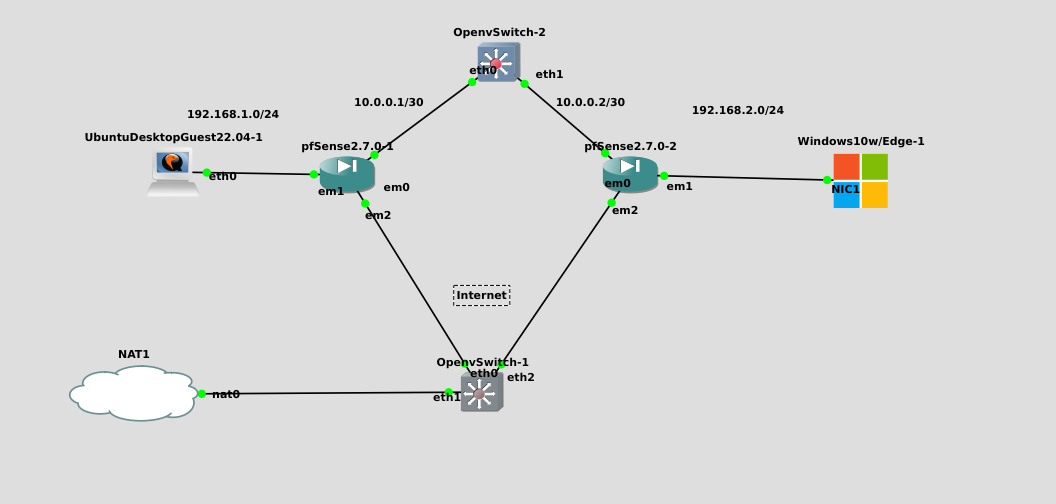
\includegraphics[scale=0.30]{00}
	\caption{Topología de red}
\end{figure}

De la topología además podemos ver las direcciones de red, las cuales son sencillas de seguir. Como punto importante, la conexión se realiza a través de la red 10.0.0.0/30, aunque se puede hacer por la otra que será marcada por el router como OPT1, que es la que permite que nuestro pfsense pueda instalar las utilidades necesarias para poder usar Wireguard. 
\vspace{5mm}

OPT1, se ha configurado con DHCP y DNS, para poder instalar Wireguard, como la instalación y configuración de interfaces conectadas a Internet está fuera de este manual no se dará más importancia más allá de que es una red de management la conectada por OPT1.

\newpage
\section{Configuración de WAN y toma de contacto con Pfsense}

Bueno el sistema es un router/firewall, el cual nos permite varias ventajas y además podemos evolucionarlo a través de paquetes como UTM. Bueno la pantalla principal se nos presenta como la siguiente:

\begin{figure}[H]
	\centering
	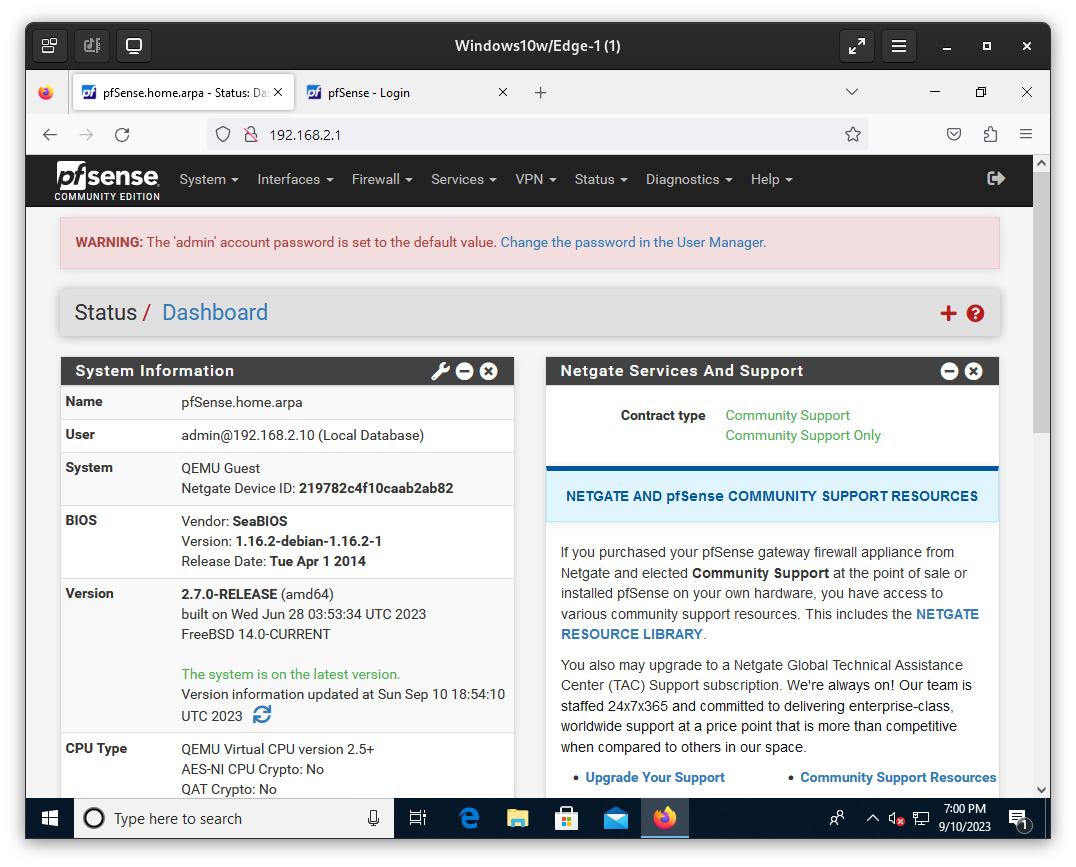
\includegraphics[scale=0.30]{01}
	\caption{Interfaz de Pfsense}
\end{figure}

Lo primero que debemos configurar son las interfaces de red básicas, porque si recordamos que tiene 3 dos de ellas las asigna automáticamente como WAN y LAN, en concreto las 2 primeras respectivamente, el router/firewall durante su instalación proveerá por defecto de una LAN 192.168.1.0/24 a todos los routers sin excepción, en mi caso como necesitamos enrutar redes privadas por PPTP de Wireguard, necesitamos que las redes sean distintas, en ese caso el segundo router/firewall DEBE tener otra subred privada diferente, esto es para poder generar unas rutas estáticas que nos permite enrutar paquetes que tengan como destino la red privada conectada.
\vspace{5mm}

Ahora la WAN debe configurarse como dirección IP estática, normalmente está todo preparado para que puedas usar DHCP para que tu proveedor de servicios o un router neutro que haga de bridge te de una dirección IP. Para ello tenemos que ir a \textbf{Interfaces -> WAN}, nos mostrará una ventana como va a aparecer en al siguiente captura, donde nos tenemos que concentrar es en: 

\begin{enumerate}
    \item IPv4 Configuration Type -> Static IPv4; Esto es para que la configuración la realicemos nosostros.
    \item IPv4 Configuaration - Aparecerá una caja nueva que nos indicará los siguientes campos:
    \begin{enumerate}
        \item IPv4 Address - Redes de máscara CIDR (Classless Inter Domain Routing) 30 - 255.255.255.252
            \begin{itemize}
                \item 10.0.0.1 - Para el router firewall conectado a Ubuntu.
                \item 10.0.0.2 - Para el router firewall conectado a Windows.
            \end{itemize}
        \item IPv4 Upstream GW -> Podemos usarlo si queremos utilizar la ruta directa sin seguridad, pero como vamos a establecer un Tunel punto a punto cifrado, lo dejamos en blanco.
    \end{enumerate}
\end{enumerate}

Una vez terminada la configuración de arriba, almacenamos las respectivas configuraciones pulsando Save.

\begin{figure}[H]
	\centering
	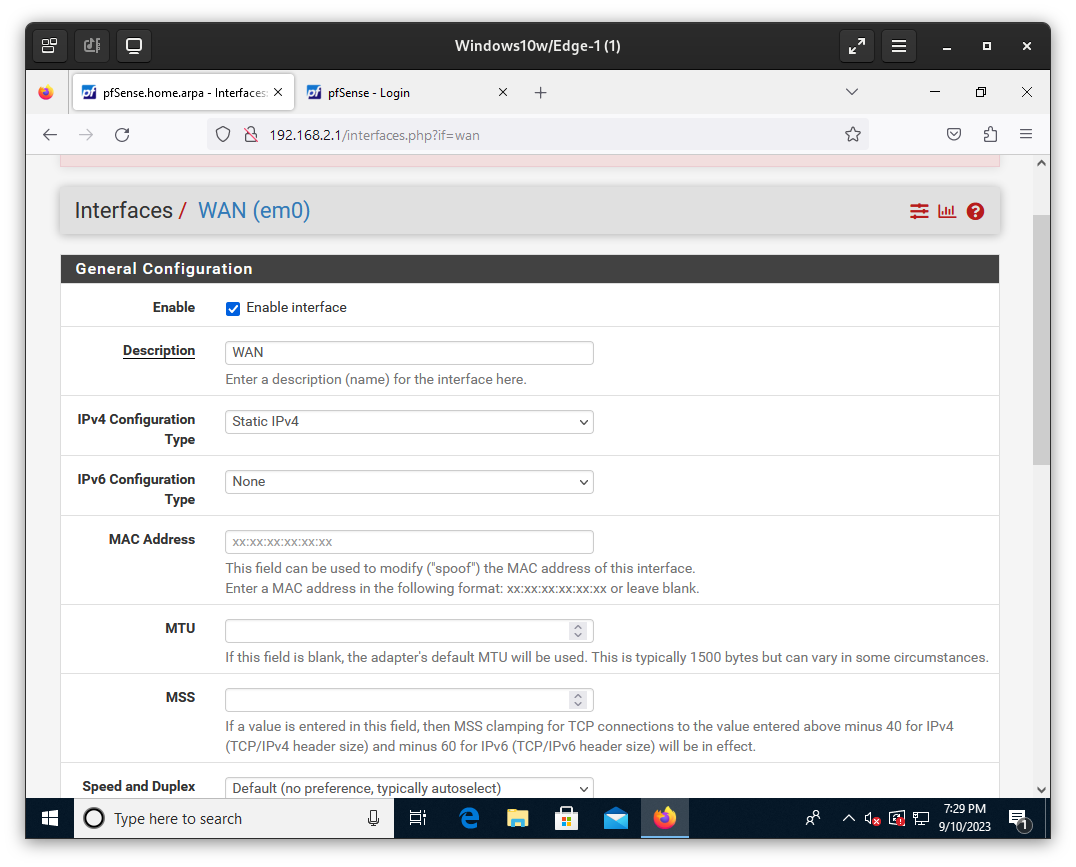
\includegraphics[scale=0.30]{02}
	\caption{Configuración de WAN}
\end{figure}

\begin{figure}[H]
	\centering
	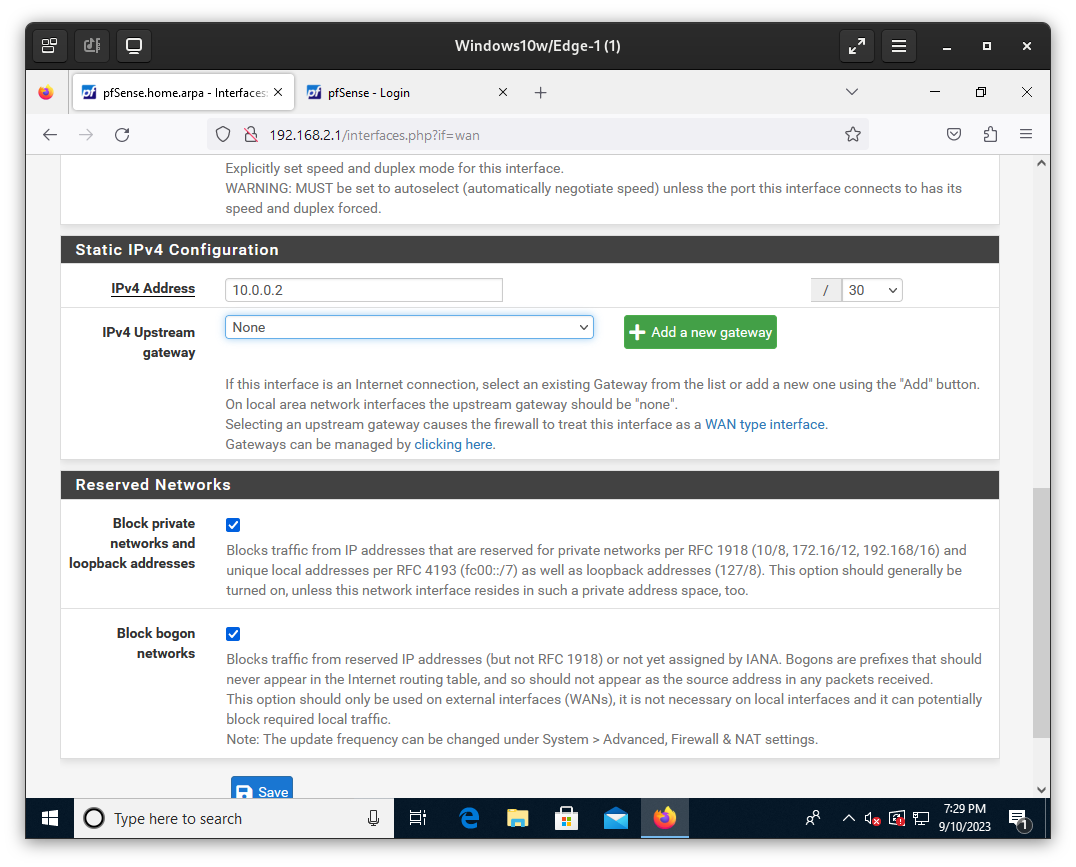
\includegraphics[scale=0.30]{03}
	\caption{Configuración de WAN - parte 2}
\end{figure}

En el otro router firewall, seguimos básicamente los mismos pasos, pero cambiando la IP.

\newpage
\section{Configuración de Wireguard}

Ahora debemos configurar Wireguard, para ello nos vamos a \textbf{VPN -> Wireguard}, luego una vez dentro tenemos que añadir un tunel en cada router/firewall. Tenemos que introducir los siguientes campos del formulario: 

\begin{enumerate}
    \item Marcar el checkbox de \emph{Enable Tunnel}.
    \item Introducir una descripción: en mi caso ponemos OFFICE1\_PPTP o OFFICE2\_PPTP.
    \item Listen Port - Podemos cambiarlo a otro que no sea el por defecto por seguridad y ofuscación. Pero para el objetivo de este manual, lo dejamos en el por defecto de Wireguard el \textbf{UDP - 51820}.
    \item Interface Keys: Aquí tenemos que generar nuevas claves pulsando el botón de la derecha y DEBEMOS guardar bien la clave pública, la privada la dejamos sin tocar y solo debe saberla el router/firewall.
\end{enumerate}

\begin{figure}[H]
	\centering
	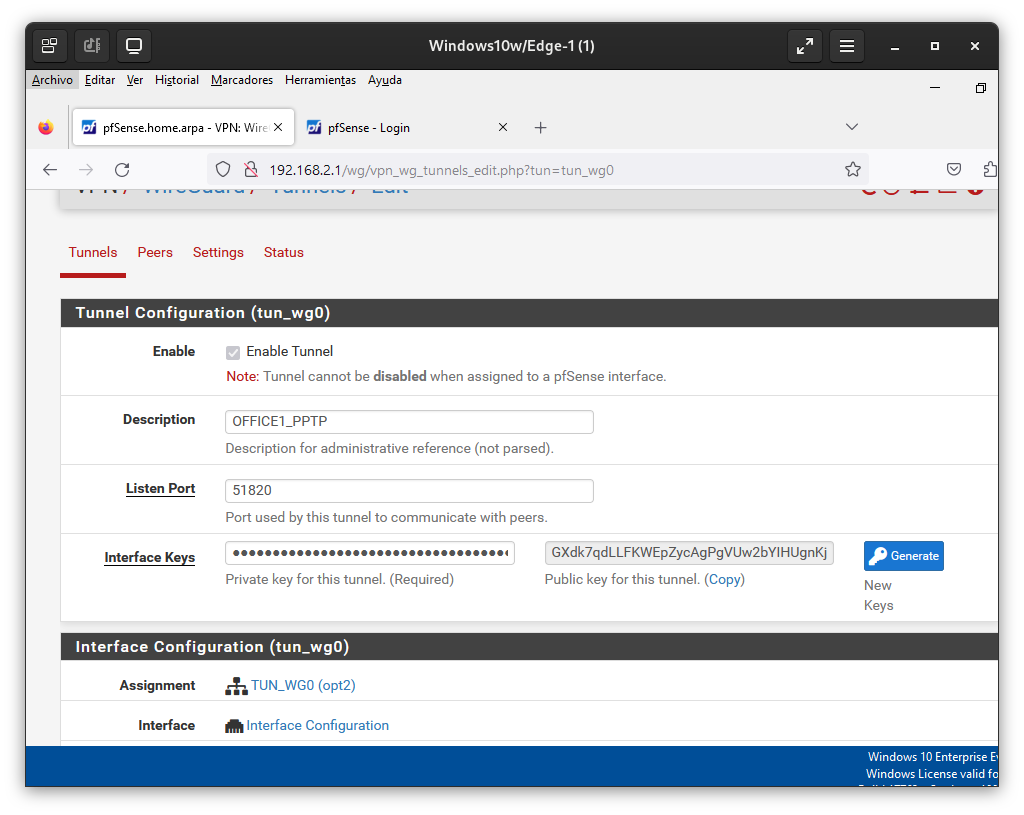
\includegraphics[scale=0.30]{05}
	\caption{Configuración del tunel de Wireguard}
\end{figure}

Una vez realizada la configuración debemos pulsar guardar y tras lo cual debemos activar el servicio de Wireguard en Settings, luego tenemos que volver al mismo tunel para permitir la asignación de la interfaz propia, es decir la dirección IP del tunel junto a su máscara. en tal caso debemos activar esa interfaz a tráves del menú de interfaces y asignarla.
\vspace{5mm}

Tenemos que poner los siguientes cambios: 

\begin{enumerate}
    \item IPv4 Configuration Type -> Static IPv4; Esto es para que la configuración la realicemos nosostros.
    \item IPv4 Configuaration - Aparecerá una caja nueva que nos indicará los siguientes campos:
    \begin{enumerate}
        \item IPv4 Address - Redes de máscara CIDR (Classless Inter Domain Routing) 30 - 255.255.255.252
            \begin{itemize}
                \item 172.16.0.1- Para el router firewall conectado a Ubuntu.
                \item 172.16.0.2 - Para el router firewall conectado a Windows.
            \end{itemize}
        \item IPv4 Upstream GW - Aquí inicializamos como puerta la dirección del otro router, esto es importante porque a pesar de su nombre, te permite crear una ruta estática hacia la otra subred privada donde estén conectados los host y servicios de otra oficina. Para crearlo debemos pulsar new Gateway que nos hará un nuevo formulario.
            \begin{itemize}
                \item 172.16.0.2- Para el router firewall conectado a Ubuntu.
                \item 172.16.0.1 - Para el router firewall conectado a Windows.
            \end{itemize}
    \end{enumerate}
\end{enumerate}

\begin{figure}[H]
	\centering
	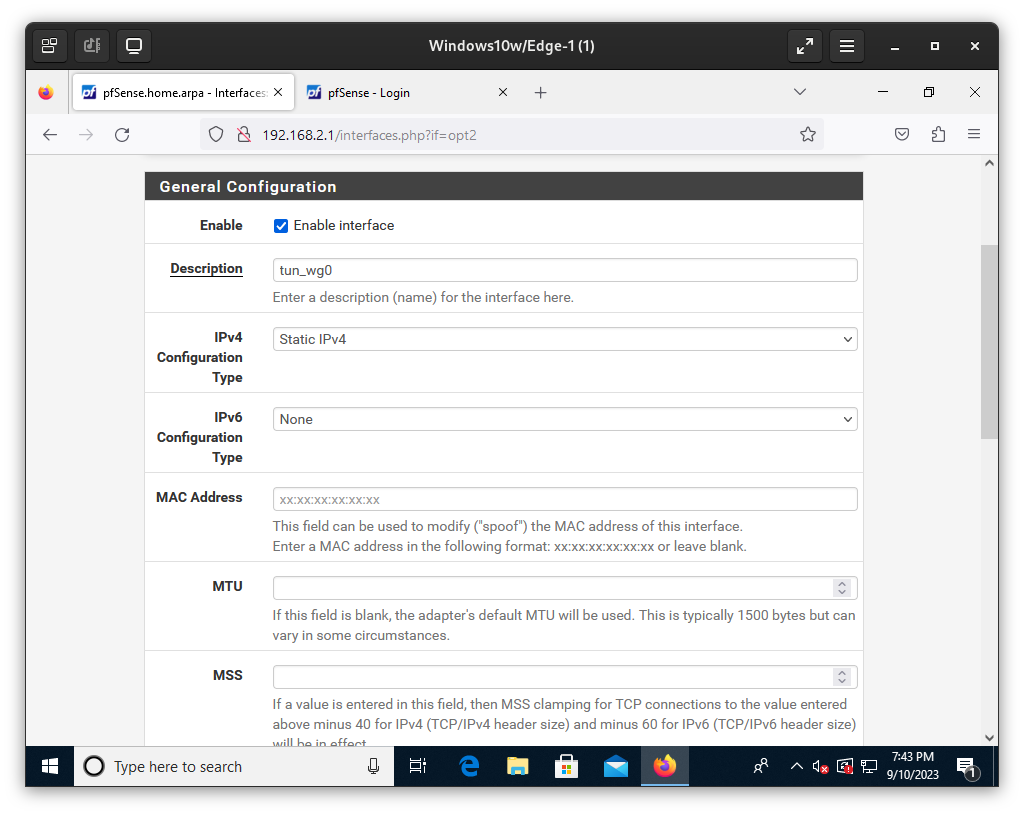
\includegraphics[scale=0.30]{06}
	\caption{Configuración de la interfaz del tunel parte 1}
\end{figure}

\begin{figure}[H]
	\centering
	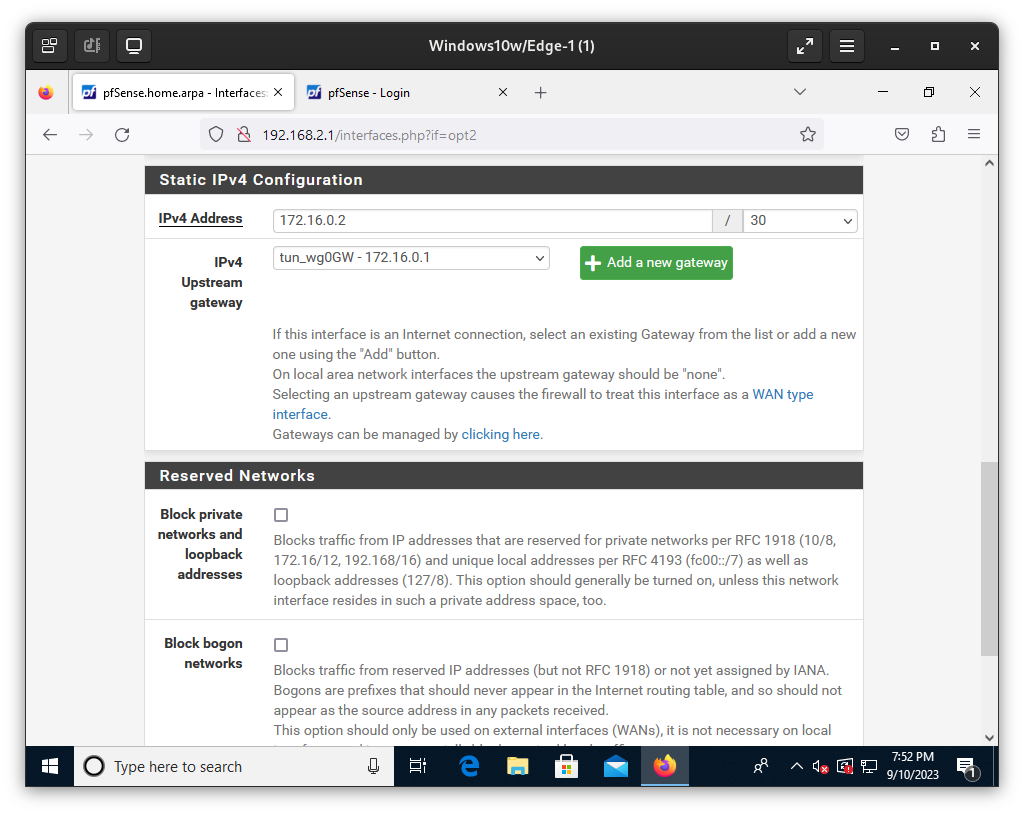
\includegraphics[scale=0.30]{07}
	\caption{Configuración de la interfaz del tunel parte 2}
\end{figure}

\begin{figure}[H]
	\centering
	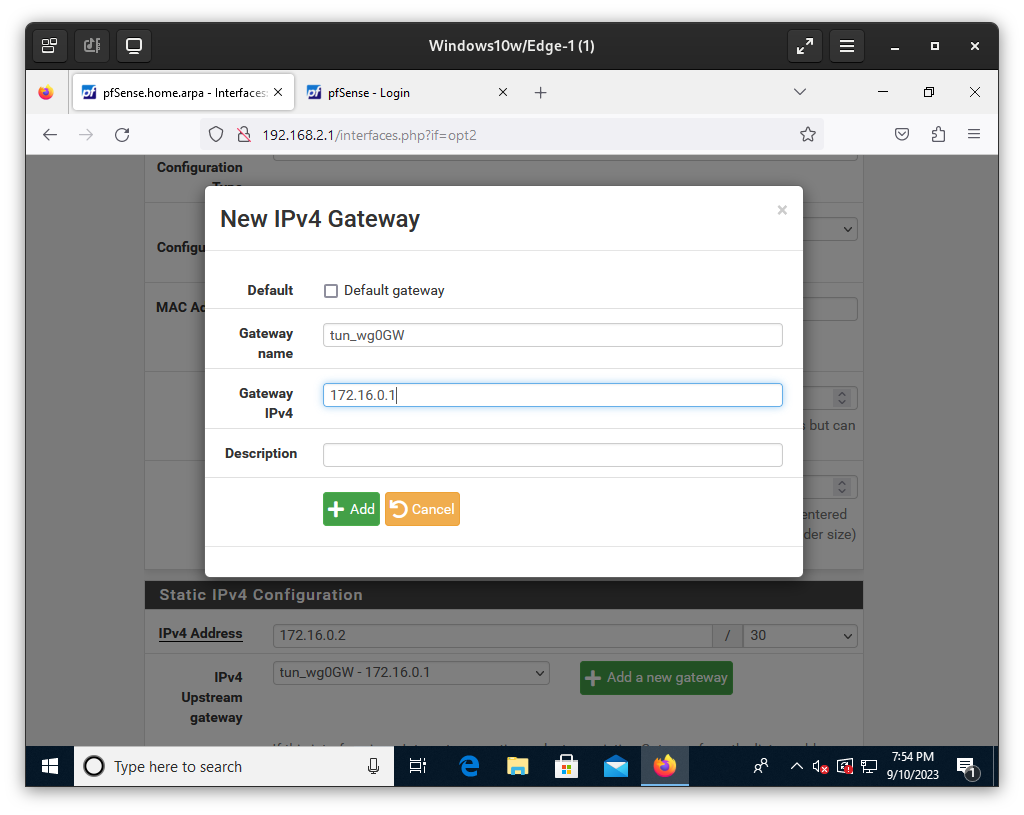
\includegraphics[scale=0.30]{08}
	\caption{Configuración de la interfaz del tunel parte 3 - Creación del Gateway}
\end{figure}

\newpage
\section{Creación de los Peer}

Ahora una vez creadas las interfaces tenemos que irnos al mismo lugar donde creamos los túneles y crear un nuevo peer, para ello debemos pulsar en Add Peer que es el icono que aparece a la derecha del tunel.

\begin{enumerate}
    \item Enable Peer - Lo marcamos.
    \item Tunnel - seleccionamos el tunel con el que queramos asociar el peer, en nuestro caso es wg0.
    \begin{enumerate}
        \item Dynamic Endpoint, lo desmarcamos porque conocemos los detalles del peer, es decir esto se suele utilizar como VPN estándar donde los clientes se conectan desde distintos puntos de Internet. En este caso nos aparecerán dos cuadros de texto.
            \begin{itemize}
                \item Endpoint - IPv4 - Introducimos la IP WAN de los routers, es decir si estamos en el router de Ubuntu, tenemos que poner la de Windows, porque es nuestro par que se conecta a ese tunel.
                \item Endpoint port - Introducimos el puerto que corresponda. si lo hemos cambiando.
            \end{itemize}
        \item KeepAlive - 1s. Es el intérvalo de los paquetes que se envían apra indicar que se mantenga la conexión abierta.
        \item Public Key - Pegamos aquí la clave pública del tunel del peer.
        \item Address Configuration - Aquí indicamos qué redes son alcanzables desde este túnel.
            \begin{itemize}
                \item 192.168.1.0/24 - Para conectar desde el router windows a Ubuntu.
                \item 192.168.2.0/24 - Para conectar desde el router Ubuntu a Windows.
                \item 172.16.0.1/32 - Para permitir la conectividad de IP del tunel desde windows a Ubuntu.
                \item 172.16.0.2/32 - Para permitir la conectividad de IP del tunel desde Ubuntu a Windows.
            \end{itemize}
    \end{enumerate}
\end{enumerate}

\begin{figure}[H]
	\centering
	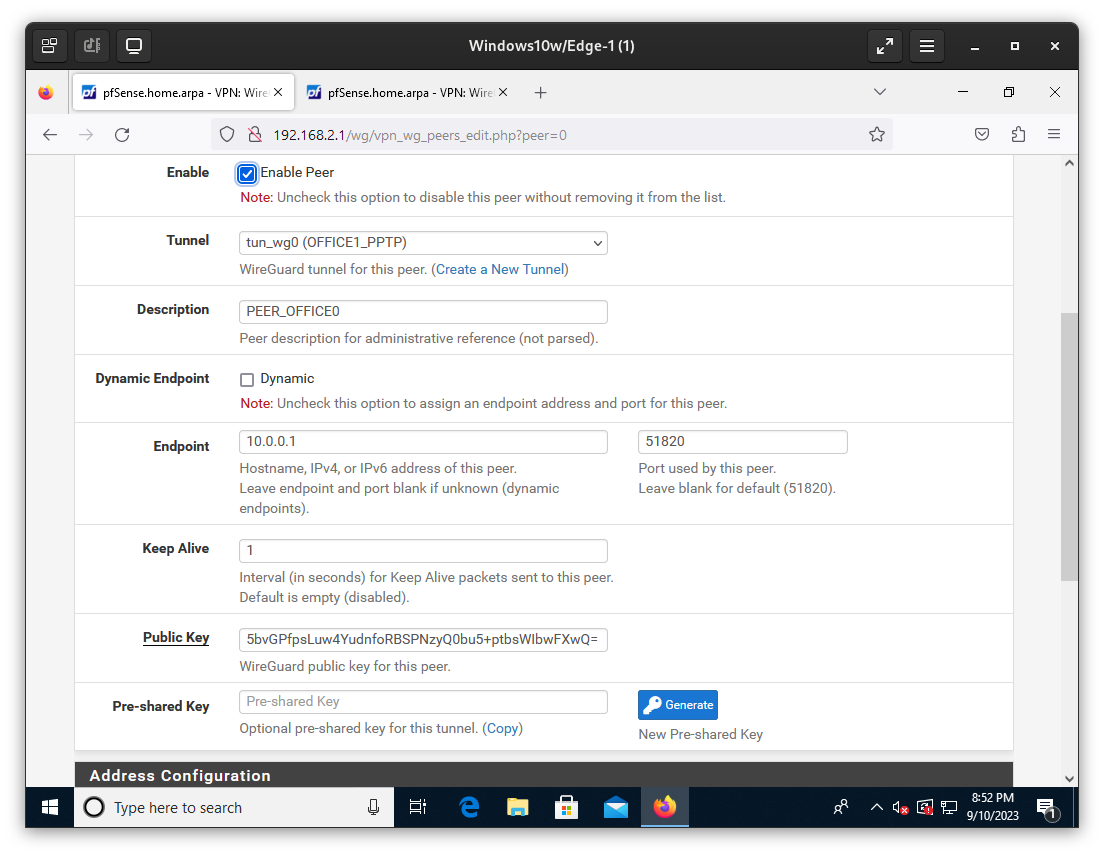
\includegraphics[scale=0.30]{09}
	\caption{Configuración del peer - De router Windows a Ubuntu}
\end{figure}

\begin{figure}[H]
	\centering
	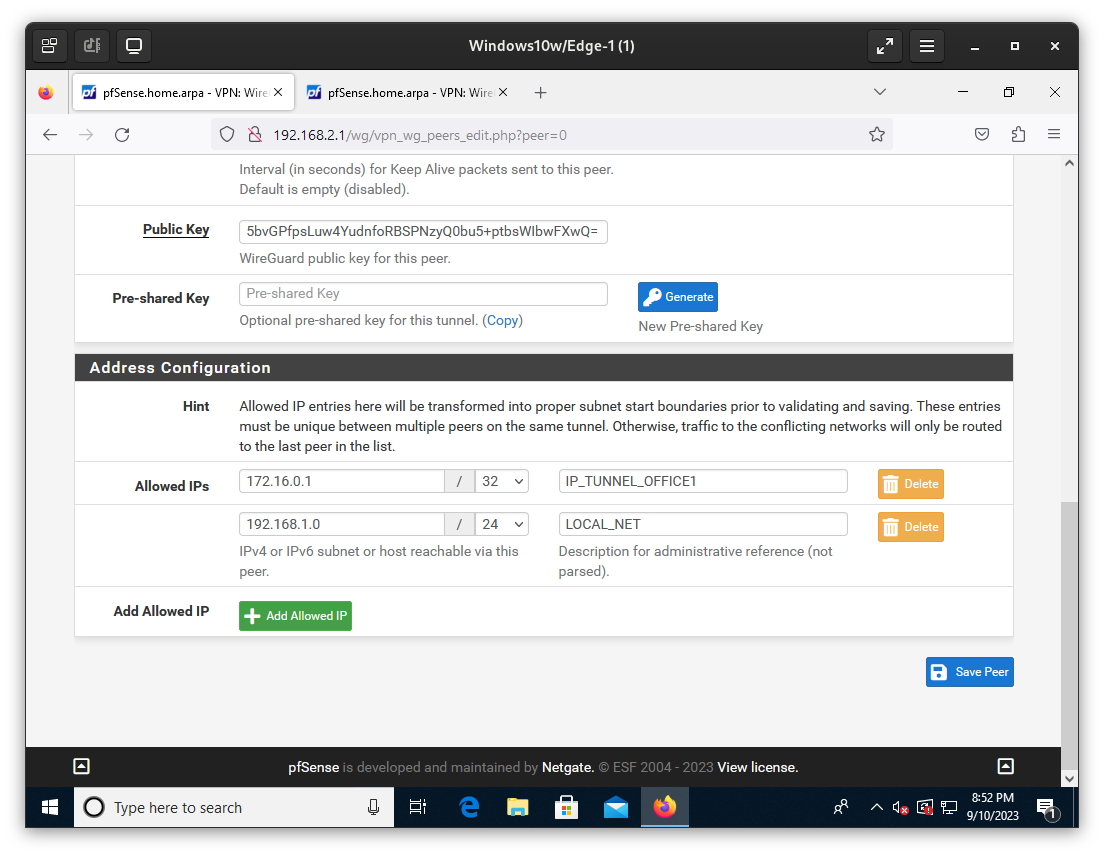
\includegraphics[scale=0.30]{10}
	\caption{Configuración del peer - De router Windows a Ubuntu - Direcciones enrutables}
\end{figure}

Ahora una vez creados los peer para los túneles, podemos ver en el estado que no se conectan, esto es porque necesitamos en la interfaz WAN una regla de firewall que permita las conexiones entrantes hacia el puerto UDP de Wireguard. las reglas son como siguen:

\begin{figure}[H]
	\centering
	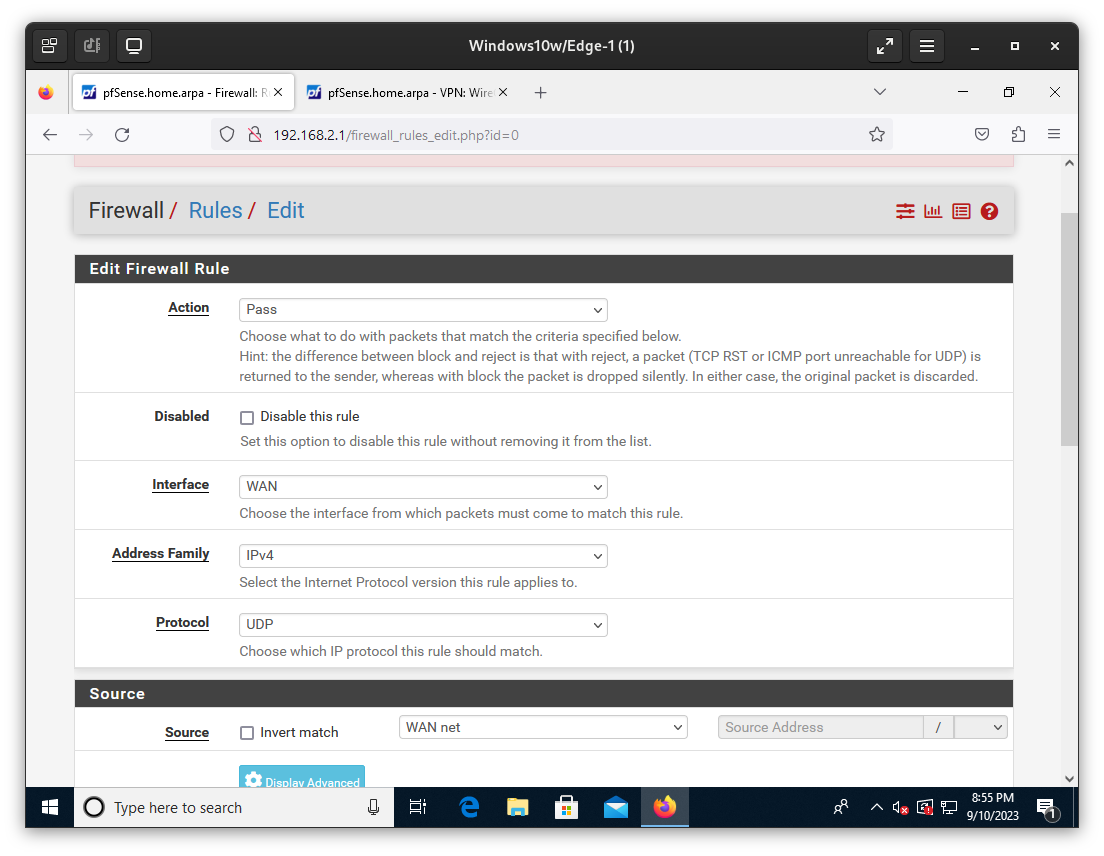
\includegraphics[scale=0.30]{11}
	\caption{Configuración de las reglas de Firewall}
\end{figure}

De estas reglas debemos tener en cuenta, que como Source debemos poner la red de la WAN, es decir toda la máscara de subred de la WAN se acepta, luego como destino tenemos que poner a este firewall. Finalmente ponemos el rango de puertos de destino con el servicio de Wireguard, el de origen es efímero.

\begin{figure}[H]
	\centering
	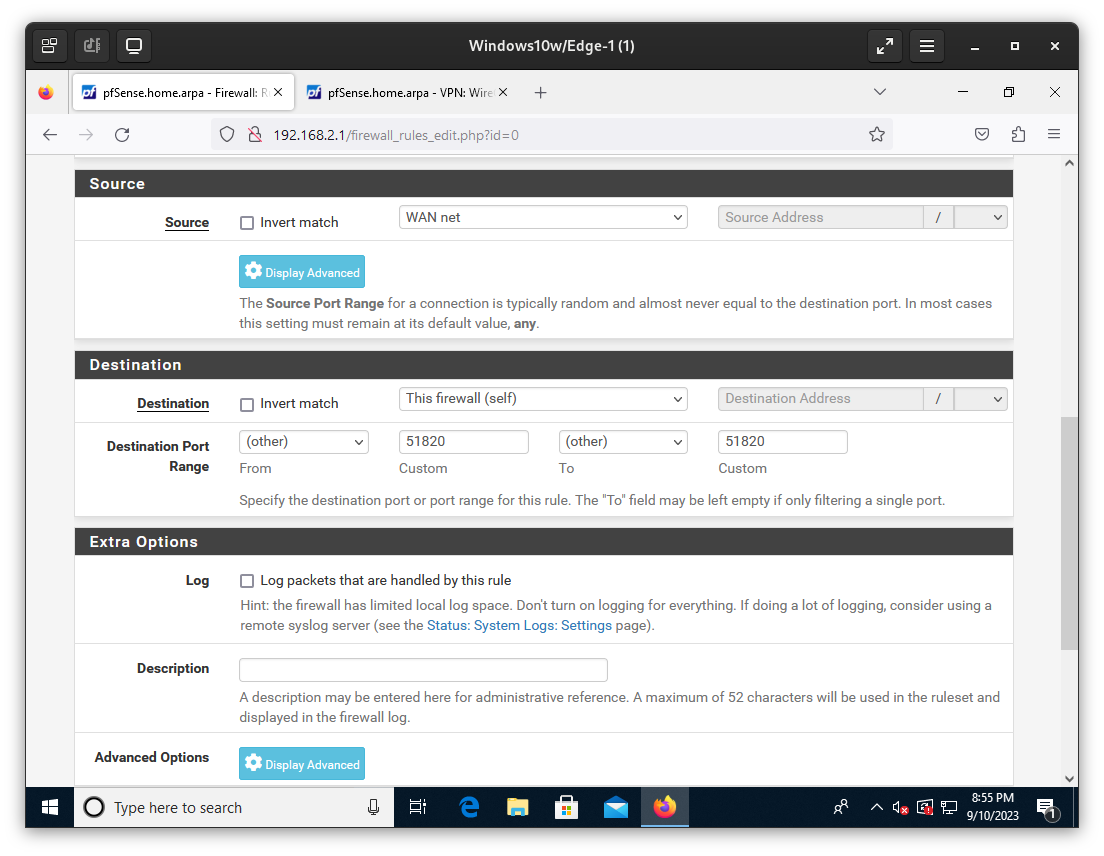
\includegraphics[scale=0.30]{12}
	\caption{Configuración de las reglas de Firewall - Parte 2}
\end{figure}

Ahora una vez que se han configurado y guardado las reglas de Firewall, podemos comprobar que la conectividad se ha realizado, porque ha cambiado la fecha del último handshake o si está conectad actualmente aparecerá en verde el handshake.

\begin{figure}[H]
	\centering
	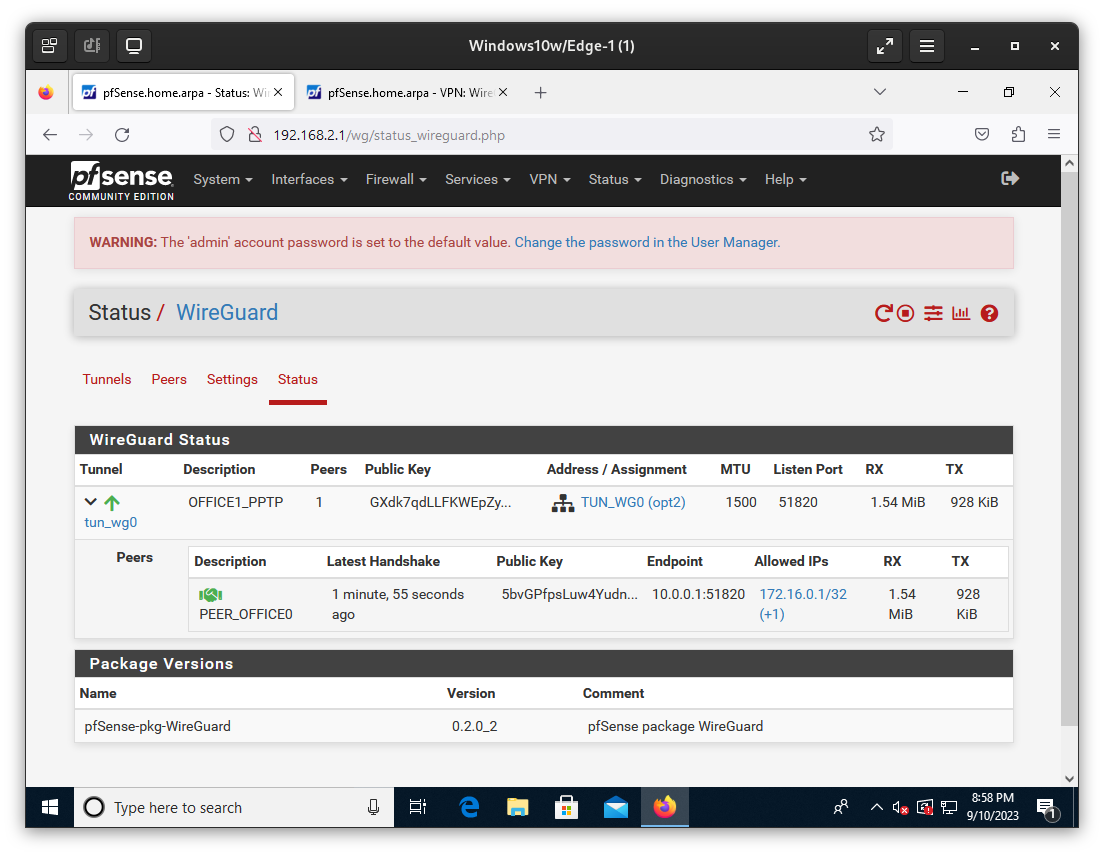
\includegraphics[scale=0.30]{13}
	\caption{handshake realizado}
\end{figure}

\newpage
\section{Configuración de ruta estática y prueba}

Por último tenemos que poner una ruta estática para poder llegar a la red privada al otro lado del tunel. Para ello tenemos que crear una ruta por el Gateway creado por el tunel anteriormente, para ello vamos a System -> Routing -> Static Routes. Creamos una nueva con la siguiente configuración.

\begin{figure}[H]
	\centering
	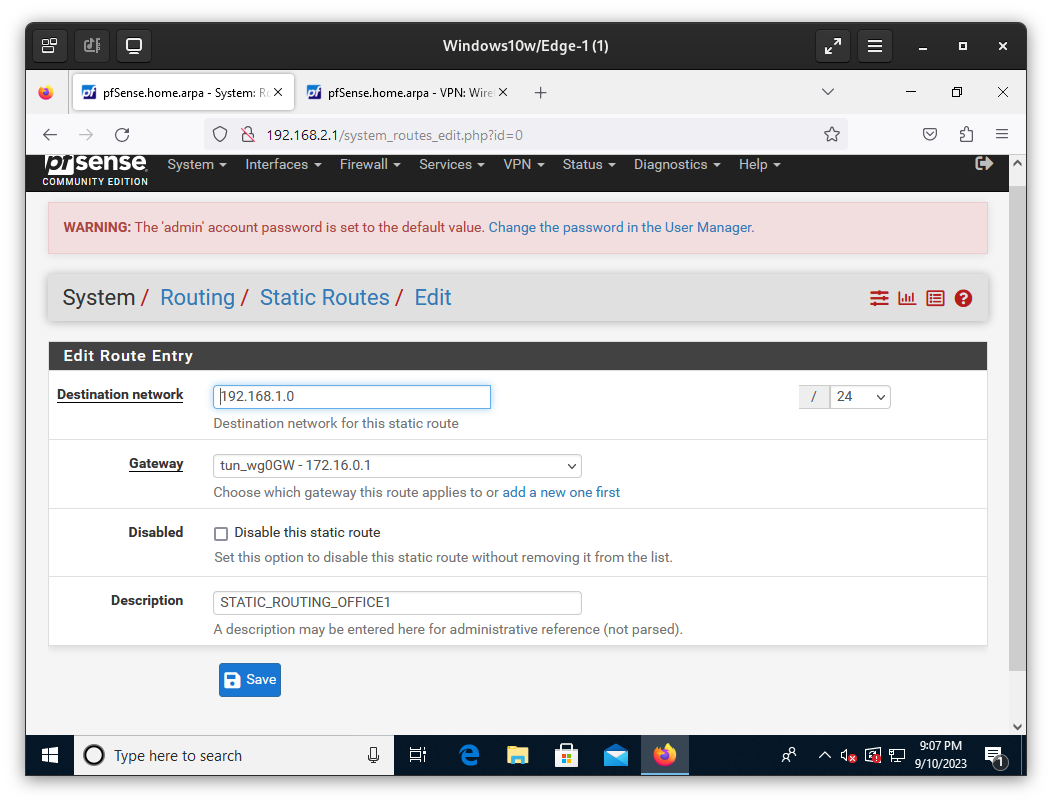
\includegraphics[scale=0.30]{14}
	\caption{Configuración de ruta estática}
\end{figure}

En el caso de que sea la red de ubuntu, tenemos que poner 192.168.2.0.
\vspace{5mm}

Como prueba se accede al otro router firewall con la IP privada de su red local. Se puede ver que accede a través del tunel porque pone la IP de acceso a la izquierda en User admin@172.16.0.2 que es la IP del tunel del equipo de Windows.

\begin{figure}[H]
	\centering
	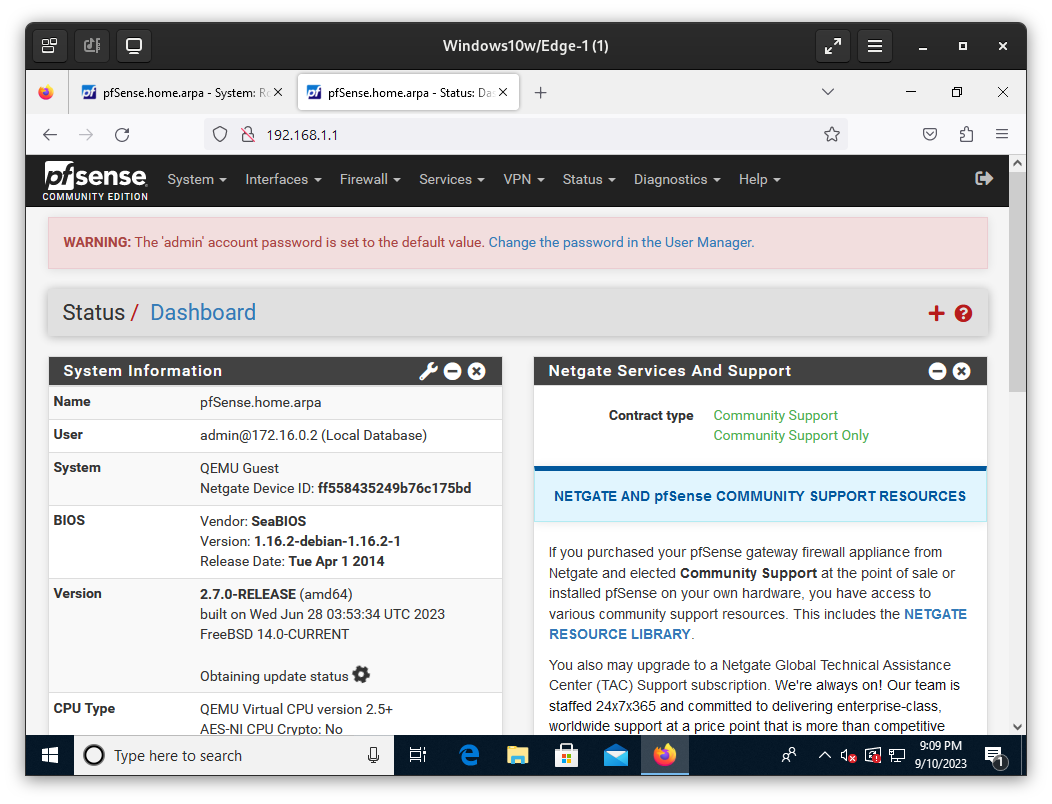
\includegraphics[scale=0.30]{15}
	\caption{Prueba}
\end{figure}

% \vspace{5mm}


% \begin{lstlisting}[style=mybash]
%     # Para una base de datos concreta
%     mysqldump --user=tiendabd --password=password --databases tiendabd --add-drop-database --add-drop-table [--replace] --host=127.0.0.1 --result-file=dump.sql
% \end{lstlisting}



%\begin{figure}[H]
%	\centering
%	\includegraphics[scale=0.30]{cuestion_1_1}
%	\caption{Se puede ver que al no haber un fallo grave, el sistema lo nota como que sigue funcionando pero en un estado degradado.}
%\end{figure}

%\newpage

%Se pueden hacer include en latex
%\newpage

\section{Section}

\subsection{Subseccion}

\subsubsection{Subseccion}



%-------Bibliografia-----------------------------

%\newpage
\section{Bibliografía}

% Ejemplo
\footnote{Administración de mdadm - Por Red Hat}
\textcolor{blue}{\url{https://access.redhat.com/documentation/en-us/red_hat_enterprise_linux/8/html/managing_storage_devices/managing-raid_managing-storage-devices#monitoring-raid_managing-raid}}



\end{document}
